\subsection{Task 2: Spatial demand and passenger spending}
Month is determined from each pickup timestamp across both source files. We count completed recorded trips with positive timestamp duration; zone maps require the relevant valid TLC zone, while directed OD analysis requires both. Reverse OD pairs remain distinct and within-zone trips are retained. The sum of all ordered OD groups equals the eligible-trip denominator in Table~\ref{tab:t2rec}.
\begin{table}[htbp]\centering\small
\caption{Task 2 denominator reconciliation. Spending counts require valid payment.}\label{tab:t2rec}
\begin{tabular}{llrrrr}\hline Month & Service & Completed & OD eligible & Spend eligible & Invalid OD \\ \hline
2026-04 & Yellow & 3,781,728 & 3,781,728 & 3,766,854 & 0 \\
2026-04 & Uber & 15,378,858 & 15,378,858 & 15,376,628 & 0 \\
2026-04 & Lyft & 5,617,095 & 5,617,095 & 5,617,090 & 0 \\
2026-05 & Yellow & 4,038,760 & 4,038,760 & 4,023,883 & 0 \\
2026-05 & Uber & 15,354,816 & 15,354,816 & 15,352,465 & 0 \\
2026-05 & Lyft & 6,770,928 & 6,770,928 & 6,770,920 & 0 \\
\hline\end{tabular}\end{table}
The eight hotspot maps use one logarithmic trip-count legend. Zone IDs 264 and 265 are valid lookup categories without drawable boundaries; their counts are preserved in the CSV. The top pickup and dropoff zones by service and month are:
\begin{itemize}
\item 2026-04 Yellow pickup: Upper East Side South (179,336), Midtown Center (161,098), Upper East Side North (158,209).
\item 2026-04 Yellow dropoff: Upper East Side North (164,064), Upper East Side South (162,183), Midtown Center (131,612).
\item 2026-04 HVFHV pickup: LaGuardia Airport (412,983), JFK Airport (318,541), Crown Heights North (270,911).
\item 2026-04 HVFHV dropoff: Outside of NYC (930,707), LaGuardia Airport (434,881), JFK Airport (378,047).
\item 2026-05 Yellow pickup: Upper East Side South (194,209), Upper East Side North (172,093), Midtown Center (158,714).
\item 2026-05 Yellow dropoff: Upper East Side North (176,133), Upper East Side South (174,281), Midtown Center (136,163).
\item 2026-05 HVFHV pickup: LaGuardia Airport (453,507), JFK Airport (365,545), Crown Heights North (283,994).
\item 2026-05 HVFHV dropoff: Outside of NYC (1,018,509), LaGuardia Airport (475,502), JFK Airport (443,360).
\end{itemize}
Figure~\ref{fig:t2hotyellow} shows the April pickup maps; the remaining six comparable maps are in the figure supplement. The twelve OD flow maps show the ten largest directed flows for each service and month, separately by trip count and passenger spending. Arrows indicate OD direction and rings show within-zone flows. The ranked CSV supplements give zone names, counts, shares, service-month denominators, valid-payment counts, totals, and means.
\begin{figure}[htbp]\centering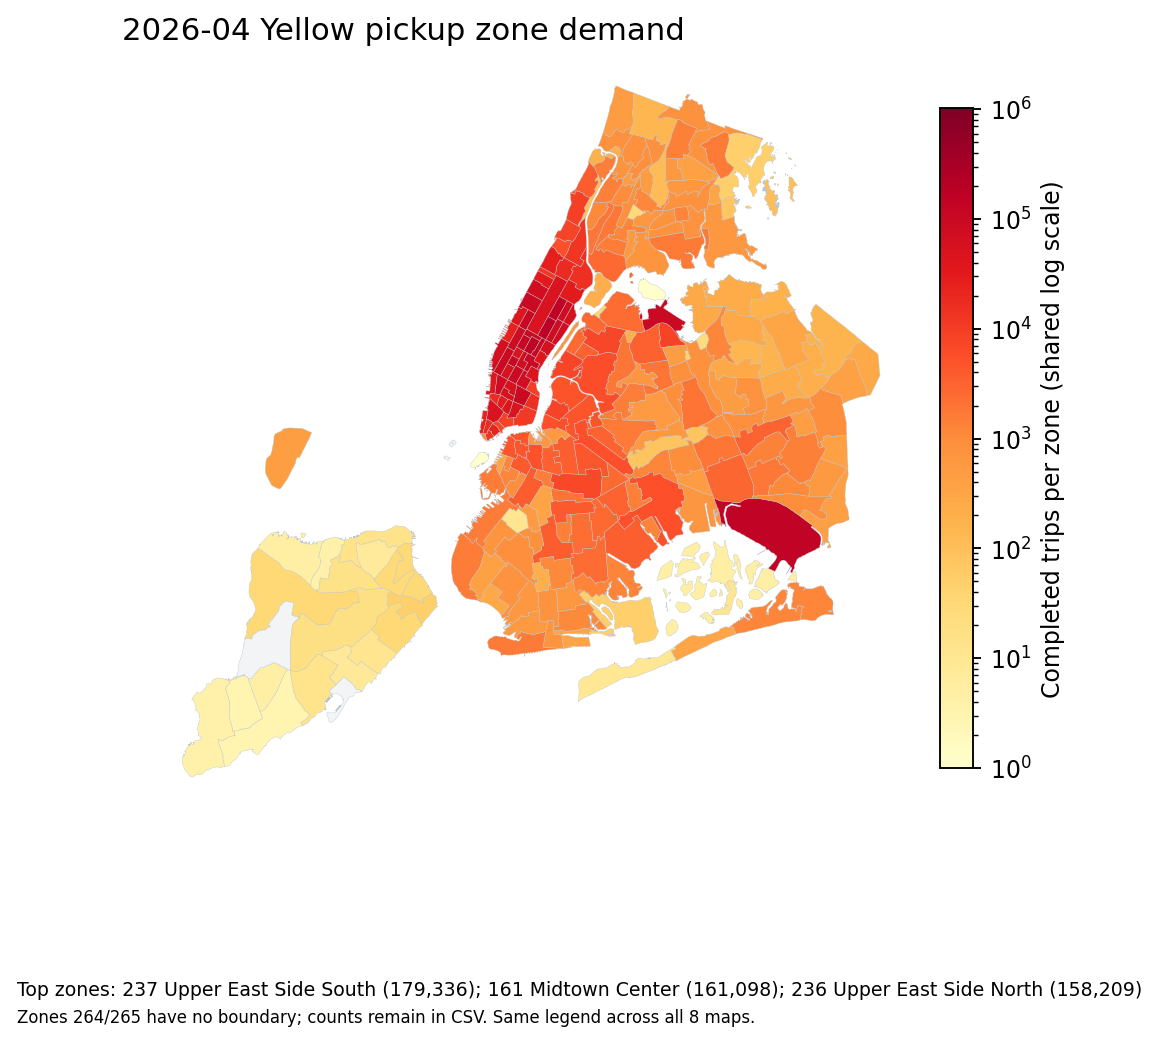
\includegraphics[width=.46\textwidth]{04_Results/Task_2/figures/hotspot_2026-04_yellow_pickup.png}\hfill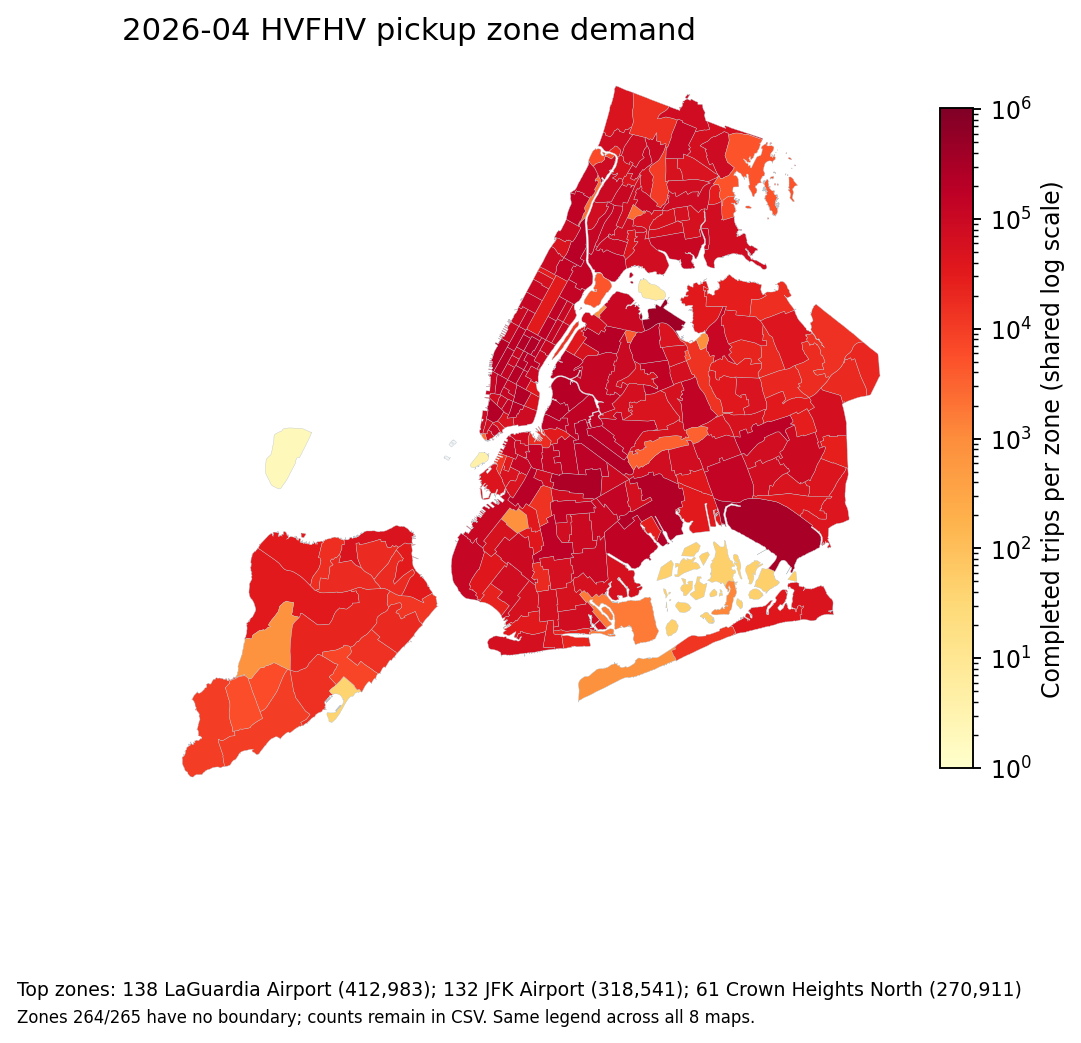
\includegraphics[width=.46\textwidth]{04_Results/Task_2/figures/hotspot_2026-04_hvfhv_pickup.png}
\caption{April pickup trip counts, Yellow and HVFHV, with a common logarithmic legend.}\label{fig:t2hotyellow}\end{figure}
\begin{figure}[htbp]\centering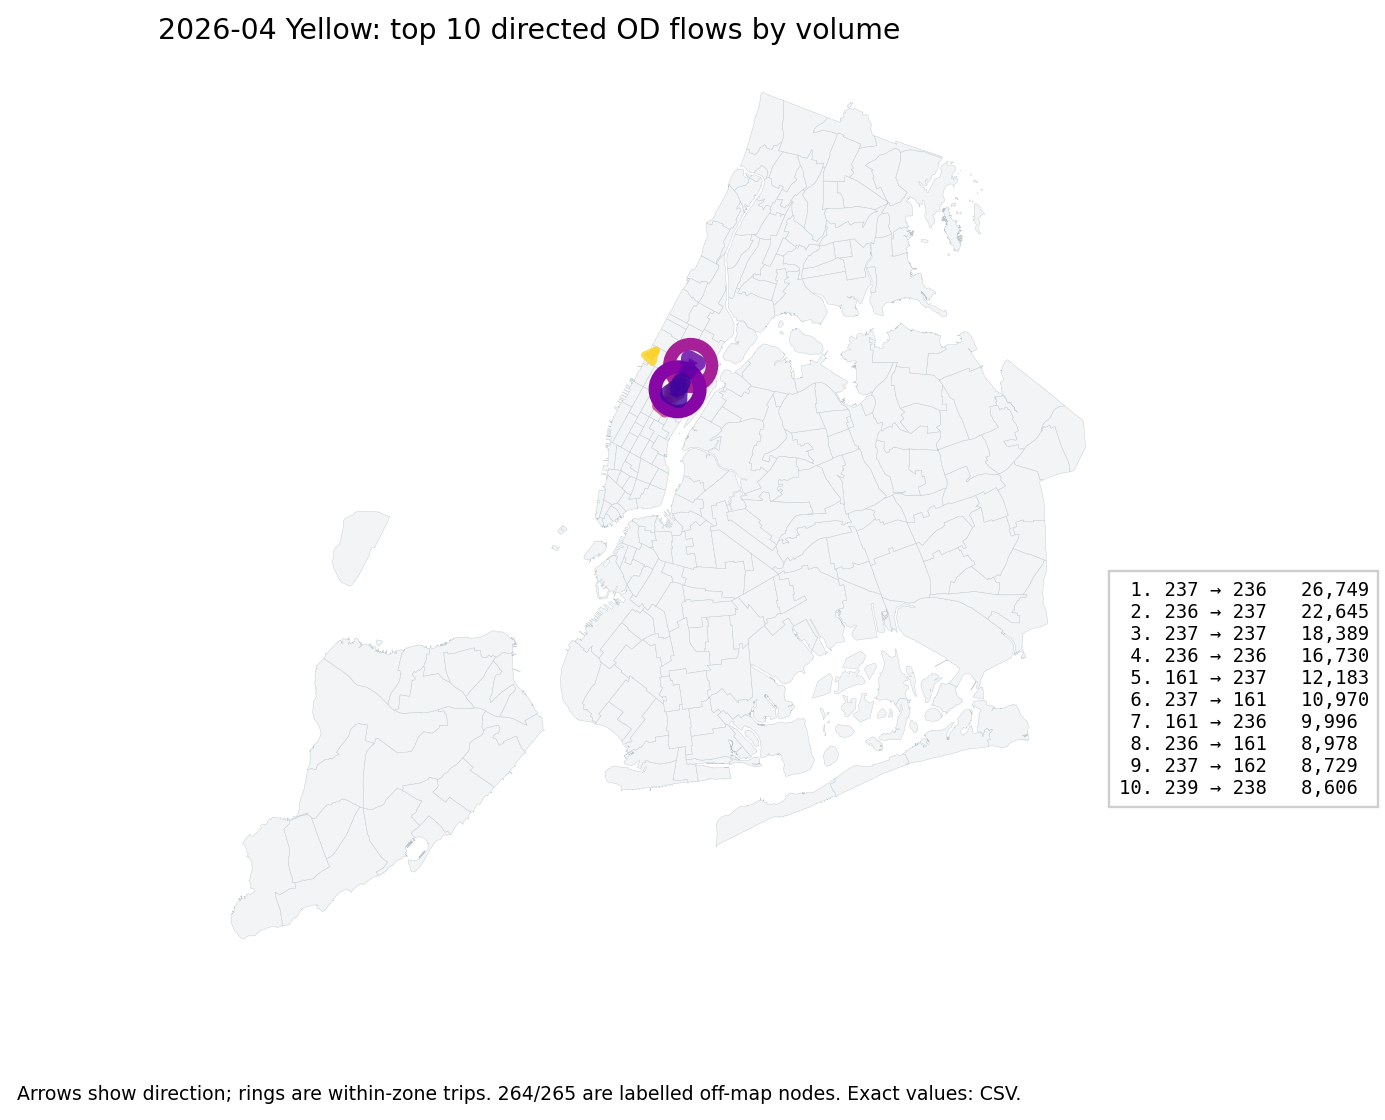
\includegraphics[width=.48\textwidth]{04_Results/Task_2/figures/od_volume_2026-04_yellow.png}\hfill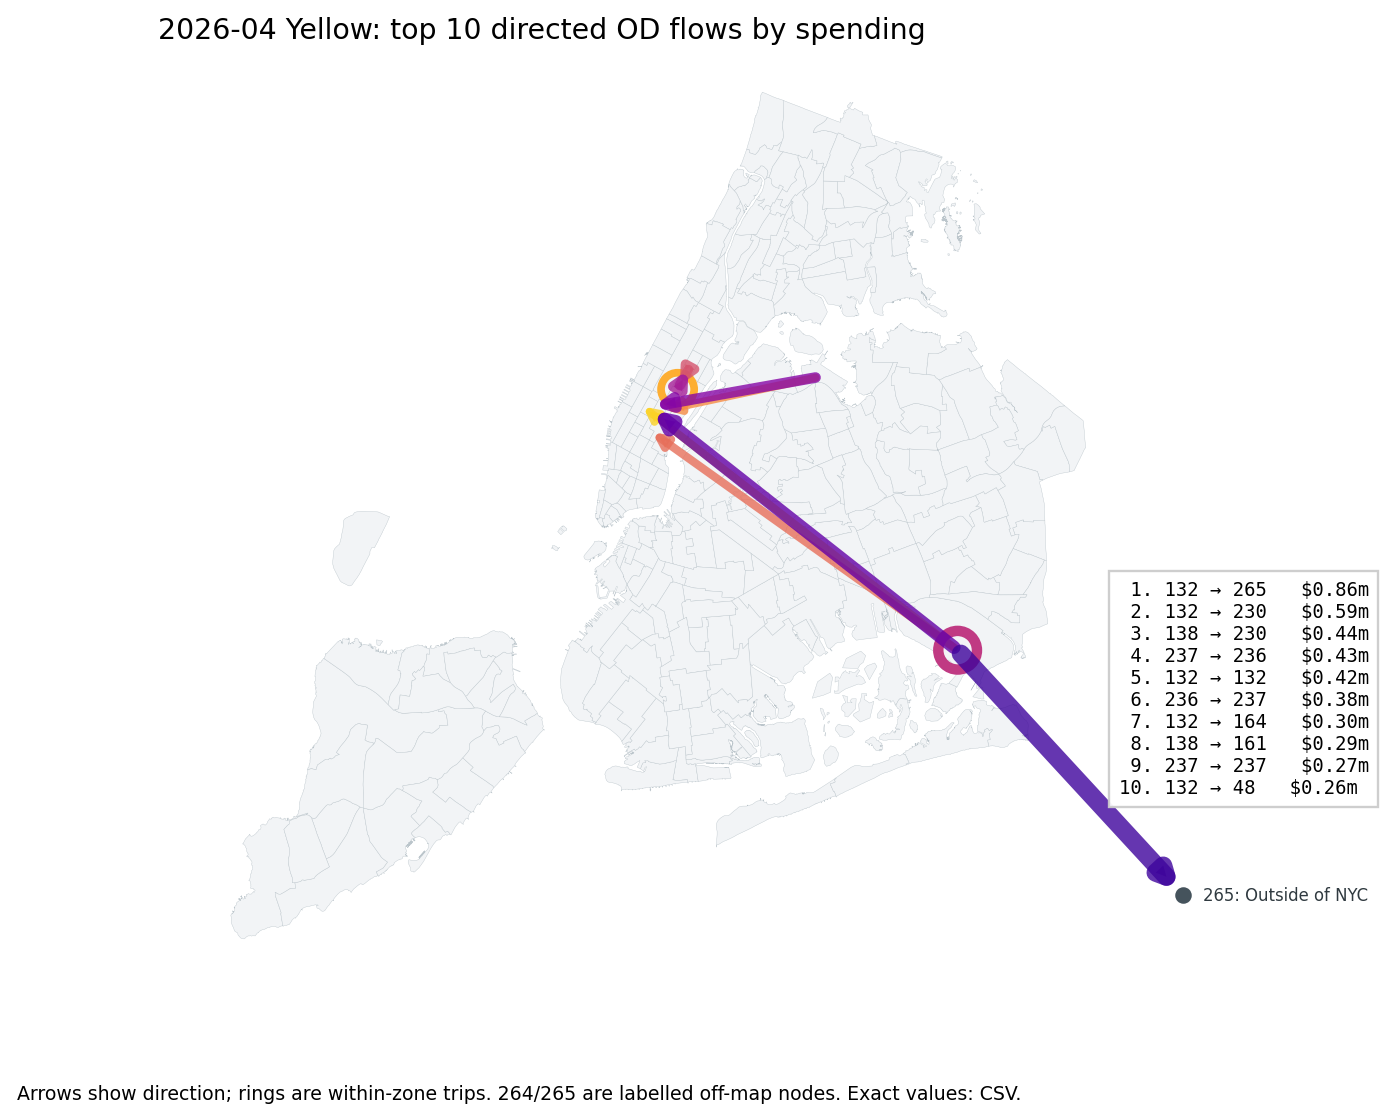
\includegraphics[width=.48\textwidth]{04_Results/Task_2/figures/od_spending_2026-04_yellow.png}
\caption{April Yellow directed flows ranked by completed trips and total recorded passenger spending.}\label{fig:t2flows}\end{figure}
\begin{table}[htbp]\centering\small\caption{Top-ten OD overlap between trip volume and total spending.}\label{tab:t2overlap}\begin{tabular}{llr}\hline Month & Service & Common OD pairs / 10 \\ \hline
2026-04 & Yellow & 3 \\
2026-04 & Uber & 2 \\
2026-04 & Lyft & 2 \\
2026-05 & Yellow & 3 \\
2026-05 & Uber & 2 \\
2026-05 & Lyft & 2 \\
\hline\end{tabular}\end{table}
\begin{table}[htbp]\centering\small\caption{Leading directed OD in each service-month: volume versus passenger spending. The full top-ten lists are in the CSV supplement.}\label{tab:t2leaders}\begin{tabular}{llrrr}\hline Month & Service & Volume leader (trips) & Spending leader (USD) & Mean USD \\ \hline
2026-04 & Yellow & 237 $\to$ 236 (26,749) & 132 $\to$ 265 (857,379) & 122.90 \\
2026-04 & Uber & 76 $\to$ 76 (57,764) & 132 $\to$ 265 (8,216,762) & 159.58 \\
2026-04 & Lyft & 76 $\to$ 76 (25,065) & 138 $\to$ 265 (2,082,850) & 132.50 \\
2026-05 & Yellow & 237 $\to$ 236 (28,964) & 132 $\to$ 265 (786,157) & 125.26 \\
2026-05 & Uber & 76 $\to$ 76 (56,166) & 132 $\to$ 265 (7,925,115) & 157.93 \\
2026-05 & Lyft & 76 $\to$ 76 (28,444) & 132 $\to$ 265 (2,836,940) & 135.64 \\
\hline\end{tabular}\end{table}
Yellow pickup and dropoff peaks remain concentrated in Upper East Side and Midtown zones in both months. HVFHV pickup peaks are LaGuardia and JFK airports, whereas its largest dropoff category is Outside of NYC (zone 265): 930,707 trips in April and 1,018,509 in May. This valid lookup category has no polygon, so the choropleth cannot color it; the count is explicit in the zone CSV and caption. Yellow's highest-volume OD is Upper East Side South $\to$ Upper East Side North (237$\to$236), while Uber and Lyft are led by an intra-zone trip (76$\to$76). Spending leaders instead connect airports to Outside of NYC, illustrating why payment ranking differs from trip ranking. Across both months, only three of Yellow's ten volume leaders and two of each platform's ten volume leaders also appear in the corresponding spending top ten. All three service-month completed-trip totals rise from April to May except Uber, which declines slightly. These comparisons describe observed completed trips and recorded payments, not total travel requests or the exact routes taken.
Yellow spending uses only \texttt{total\_amount}; HVFHV spending sums base fare, tolls, BCF, sales tax, congestion surcharge, airport fee, tips, and CBD congestion fee, excluding driver pay. A missing/nonfinite component makes the trip's spending undefined; we never replace it with zero. Negative total spending is excluded as a likely refund or correction. Values above USD 1,000 are audited but retained because they can represent long trips. Yellow cash tips may not be recorded. The flow maps show zone-centroid associations or labelled off-map nodes, not actual routes; demand represents completed trip records rather than all requests.
